%
% main.tex - a typical phil presentation
%
% Copyright (c) 2011, Phil Maker
% 
% All rights reserved.
%    
\documentclass{beamer}
%\documentclass[a4paper,handout]{beamer}
%\usepackage{pgfpages}
%\pgfpagesuselayout{4 on 1}[a4paper,border shrink=5mm]
\mode<presentation>{\usetheme{Pjm}}
\usepackage{graphics}
\usepackage{fancyvrb}
\usepackage[english]{babel}
\usepackage[latin1]{inputenc}
\usepackage{hyperref}
\definecolor{links}{HTML}{2A1B81}
\hypersetup{
  pdftitle = {Alaska 2014: Energy Storage Talk},
  pdfsubject = {Energy Storage in AU/AQ}
  pdfkeywords = {Energy, Renewables, Powerwater, Phil Maker},
  pdfauthor = {\textcopyright\ Phil Maker},
  pdfcreator = {\LaTeX\ with package \flqq hyperref \frqq},
  colorlinks,linkcolor=,urlcolor=links
}
%\usepackage{multimedia} % for movie's later on

\title{Energy Storage in Remote Australia: \\
  conniptions and kerfuffles}
\author{Phil Maker \href{mailto:philip.maker@gmail.com}{\texttt{<philip.maker@gmail.com>}}}
\institute{ACEP/Powerwater Remote Operations}
\date{March 2014}
\logo{
\includegraphics[height=0.7cm]{logo.jpg}}
\begin{document}
\begin{frame}
  \maketitle
  \vspace{-1.2cm}
  \begin{abstract}
    \small A review of energy storage in hybrid systems in Remote Australia
    including the messy bits (well a wee bit at least).
  \end{abstract}
\end{frame}

\section{Overview}
\begin{frame}\frametitle{Where: Australia}
\begin{columns}
\begin{column}{7cm}
  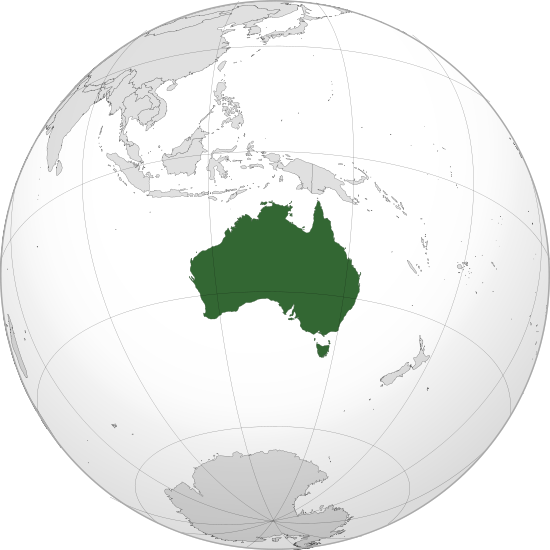
\includegraphics[width=6cm]{AU.png}
\end{column}
\begin{column}{5cm}\it
\href{http://www.kiplingsociety.co.uk/poems_serving.htm}{``I keep six honest serving men,
They taught me all I knew,
Their names are What and Why and When
And How and Where and Who.''} -- \href{http://en.wikipedia.org/Rudyard_Kipling}{Kipling}
\pause
\begin{itemize}
\item Energy storage in NT/WA.\pause
\item And the conniptions and kerfuffles (see handbook).\pause
\item Feel free to interrupt or redirect me.
\end{itemize}
\end{column}
\end{columns}
\end{frame}

\section{Northern Territory}
\begin{frame}\frametitle{Northern Territory/\href{http://www.powerwater.com.au}{Powerwater}}
\begin{columns}
\begin{column}{5cm}
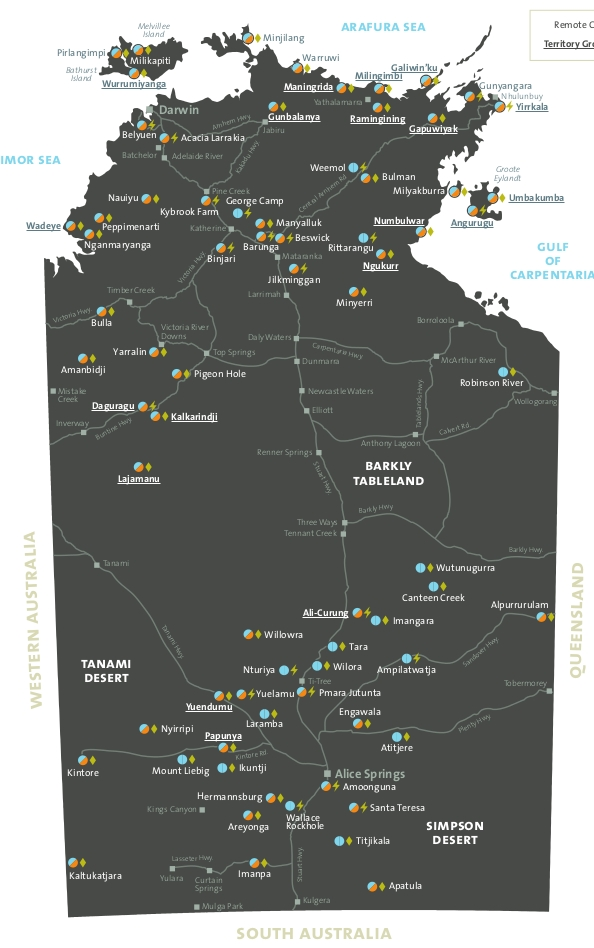
\includegraphics[width=5cm]{PW_map_section_A4.jpg}
\end{column}
\begin{column}{6cm}
  \begin{itemize}
  \item Early \href{http://www.sma.de/en.html}{SMA} systems for delaying gen switch up (20y lifetime).
  \item Small ($\approx$ 50kW) PV/Wind systems.
  \item Concentrated PV with limited smoothing.
  \item \href{http://www.epuron.com.au/project/tkln}{Ti Tree, Kalkarindji and Lake Nash} ($\approx$ 1MW total PV, 80\%
    peak penetration).
  \item \href{http://www.powerwater.com.au/solardiesel}{ASIM and Solar Diesel Handbook.}
  \item Medium Pen Rollout.
  \item High Pen Diesel off systems.
  \end{itemize}
\end{column}
\end{columns}
\end{frame}

\section{Western Australia}
\begin{frame}\frametitle{Western Australia/Horizon Power, Verve Energy}
In the past:
\pause
\begin{itemize}
\item Wind Diesel systems using Enercon, Vestas and Vergnet WTGS.
\pause
\item Low Load Diesels: 12L/hr at 7\% load for 320kW generator which
gives us 280kW of spinning reserve and 190kW of step load.
\pause
\item Flywheel Energy Storage: 18MWs at 500kW so 36s at rated which is
  enough to start and synchronise a diesel.
\pause
\end{itemize}
\pause
Currently:
\begin{itemize}
\item \href{http://www.horizonpower.com.au/documents/TECHNICAL_REQUIREMENTS_FOR_RENEWABLE_ENERGY_SYSTEMS___LOW_VOLTAGE_NETWORK3548309.PDF}{PV with hosting
capacity limits and mandatory battery smoothing}.
\pause
\item Its very hard to get some of them away from Low Load diesels :-).\pause
\item But I'm sure something will happen.
\end{itemize}
\end{frame}

\section{Some obvious facts?}
\begin{frame}\frametitle{Some obvious facts?}
  \begin{itemize}
  \item A standby loss of $x>k$ kW is a show stopper!\pause

    For example a 500kW for 36s flywheel is useless because its 
    standby losses might be 15kW.\pause

    \textbf{Complete piffle: just resize your PV array by 30kW ($<$10\%) and have a 
    a brandy, its not the standby loss, its the CAPEX/Engineering}\pause
  \item Round trip efficiency is important.\pause
    Well perhaps but if you can give me a cheap 500kW solution with 50\%
    round trip efficiency I'm going to buy it.\pause
  \item Its about energy and load shifting.\pause
    A bit, it turns out that most of our NT work will be power limited using 
    East/West arrays (or tracking). 
  \end{itemize}
\end{frame}

\section{Our Past Mistakes}
\begin{frame}\frametitle{Our Past Mistakes}
So what have your mob got wrong:\pause
  \begin{itemize}
  \item TKLN - an award winning design that flogs batteries for no real reason.\pause

    Well we do not use the diesel spinning reserve as a resource.\pause
  \item Concentrated Solar that is not intergrated in the power system.\pause
  \item No Low Load Diesels.\pause

    Note that running diesels at low load is impossible and anyone who
    suggests it is a liar and a coward.\pause
  \item And difficulties in sizing sets for loads.
  \end{itemize}
  
\end{frame}

\section{Our Future Mistakes}
\begin{frame}\frametitle{Our Future Mistakes}
So our cunning plans are:
  \begin{itemize}
  \item We've done a few design studies and a wee bit of modelling.\pause
  \item Expecting to use a 30m..2h Li Ion battery system with diesel off 
    capability.\pause
    That is we need a power battery, we are not doing load shifting.\pause
  \item Roll out medium penetration first and prove to our operations people 
    that high penetration can work.\pause
  \item Continue working on a variety of projects in order to improve
    system performance.
  \end{itemize}
\end{frame}

\section{So..}
\begin{frame}\frametitle{So what!}
  \begin{itemize}
  \item Share our lessons learnt in a frank fashion.\pause
  \item Chemistry is difficult.\pause
  \item Its not just the technology.\pause
  \item Don't look at the problem just from your interests, e.g. in my case
    control systems.\pause
  \item Try to replicate projects/share risks,\pause
    particularly with remote battery chemistry.
  \end{itemize}

\vfill
  \begin{quote}
``Learning is not compulsory... \par\pause
neither is survival'' -- W. Edwards Deming
  \end{quote}
\end{frame}
\end{document}

